\documentclass{beamer}
\usepackage{beamerthemeSingapore}
\usepackage[T1]{fontenc}
\usepackage{amsmath}
\usepackage[brazil]{babel}
\usepackage[utf8x]{inputenc}
\usepackage{multimedia}
\usepackage{graphicx}
\usepackage{color}
\usepackage{multirow}


\def\abovestrut#1{\rule[0in]{0in}{#1}\ignorespaces}
\def\belowstrut#1{\rule[-#1]{0in}{#1}\ignorespaces}
\def\abovespace{\abovestrut{0.20in}}
\def\aroundspace{\abovestrut{0.20in}\belowstrut{0.10in}}
\def\belowspace{\belowstrut{0.10in}}

\newcommand{\Lum}{\textit{Simple}}
\newcommand{\Ldois}{\textit{Time}}
\newcommand{\Ltres}{\textit{Variance}}
\newcommand{\Lquatro}{\textit{Movie}}
\newcommand{\Lcinco}{\textit{Complex}}


\newcounter{headercounter}

\newcommand{\header}[1]{
  \addtocounter{headercounter}{1}
  {\Huge
    \begin{center}
      \textbf{ #1}
    \end{center}
}
}

\title{On the Use of Hard and Soft Reservation Schemes in Constant Bandwidth Servers}
\author{Alexandre Passos, George Lima}
\date{WTR 2009}
\institute{DCC-UFBA}

\begin{document}

\maketitle

\begin{frame}
  \frametitle{Contents}
  \begin{itemize}
  \item Hard/soft reservation
  \item Possible metrics
    \begin{itemize}
    \item Response time
    \item Jitter
    \item Deadline miss ratio
    \item Wait time
    \end{itemize}
  \item Our simulations
  \item Conclusions
  \end{itemize}
\end{frame}

\begin{frame}
  \frametitle{Hard/soft reservation}
  
  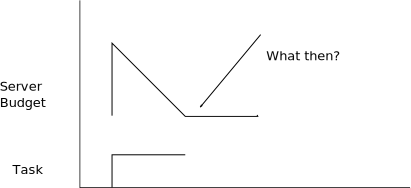
\includegraphics{hardvsoft}
\end{frame}

\begin{frame}
  \frametitle{Hard/soft reservation}
  
  \begin{tabular}[t]{rcl}
    Hard reservation &$\rightarrow$& wait until next period \\  
    Soft reservation& $\rightarrow$& recharge budget now with a lower deadline
  \end{tabular}

\vspace{2cm}
  In both cases the system remais schedulable. The only difference is
  which is better for performance.

\end{frame}


\begin{frame}
  \frametitle{Defining ``better''}
  
  There is no right answer:
\vspace{0.5cm}

  \begin{tabular}[t]{rp{7cm}}
    Response time & If it takes less time, on average, with one
    server, use that \\
    Jitter & If the response time of one server is more predictable,
    use that one \\
    Deadline miss ratio & If the tasks running under one server miss
    less deadlines than the tasks running on the other server, the
    former might be better \\
    Wait time & If the tasks running on one server tend to wait less
    time to execute, then this server might be better
  \end{tabular}
  
\end{frame}

\begin{frame}
  \frametitle{Our simulations}
  \framesubtitle{The goal}
  
  To find simple and yet representative scenarios where we could
  benchmark those metrics on soft and hard CBS servers.
\end{frame}

\begin{frame}
  \frametitle{Our simulations}
  \framesubtitle{Scenarios}

  A hard real-time background task with constant period and cost and
  one (or more) foreground CBS servers running predefined traces. We
  then compare the results of hard and soft CBS for each scenario.
\end{frame}

\begin{frame}
  \frametitle{Our simulations}
  \framesubtitle{Scenarios}
  \begin{itemize}
  \item \Lum{}: The simplest possible: normally distributed with a low variance
  \end{itemize}
  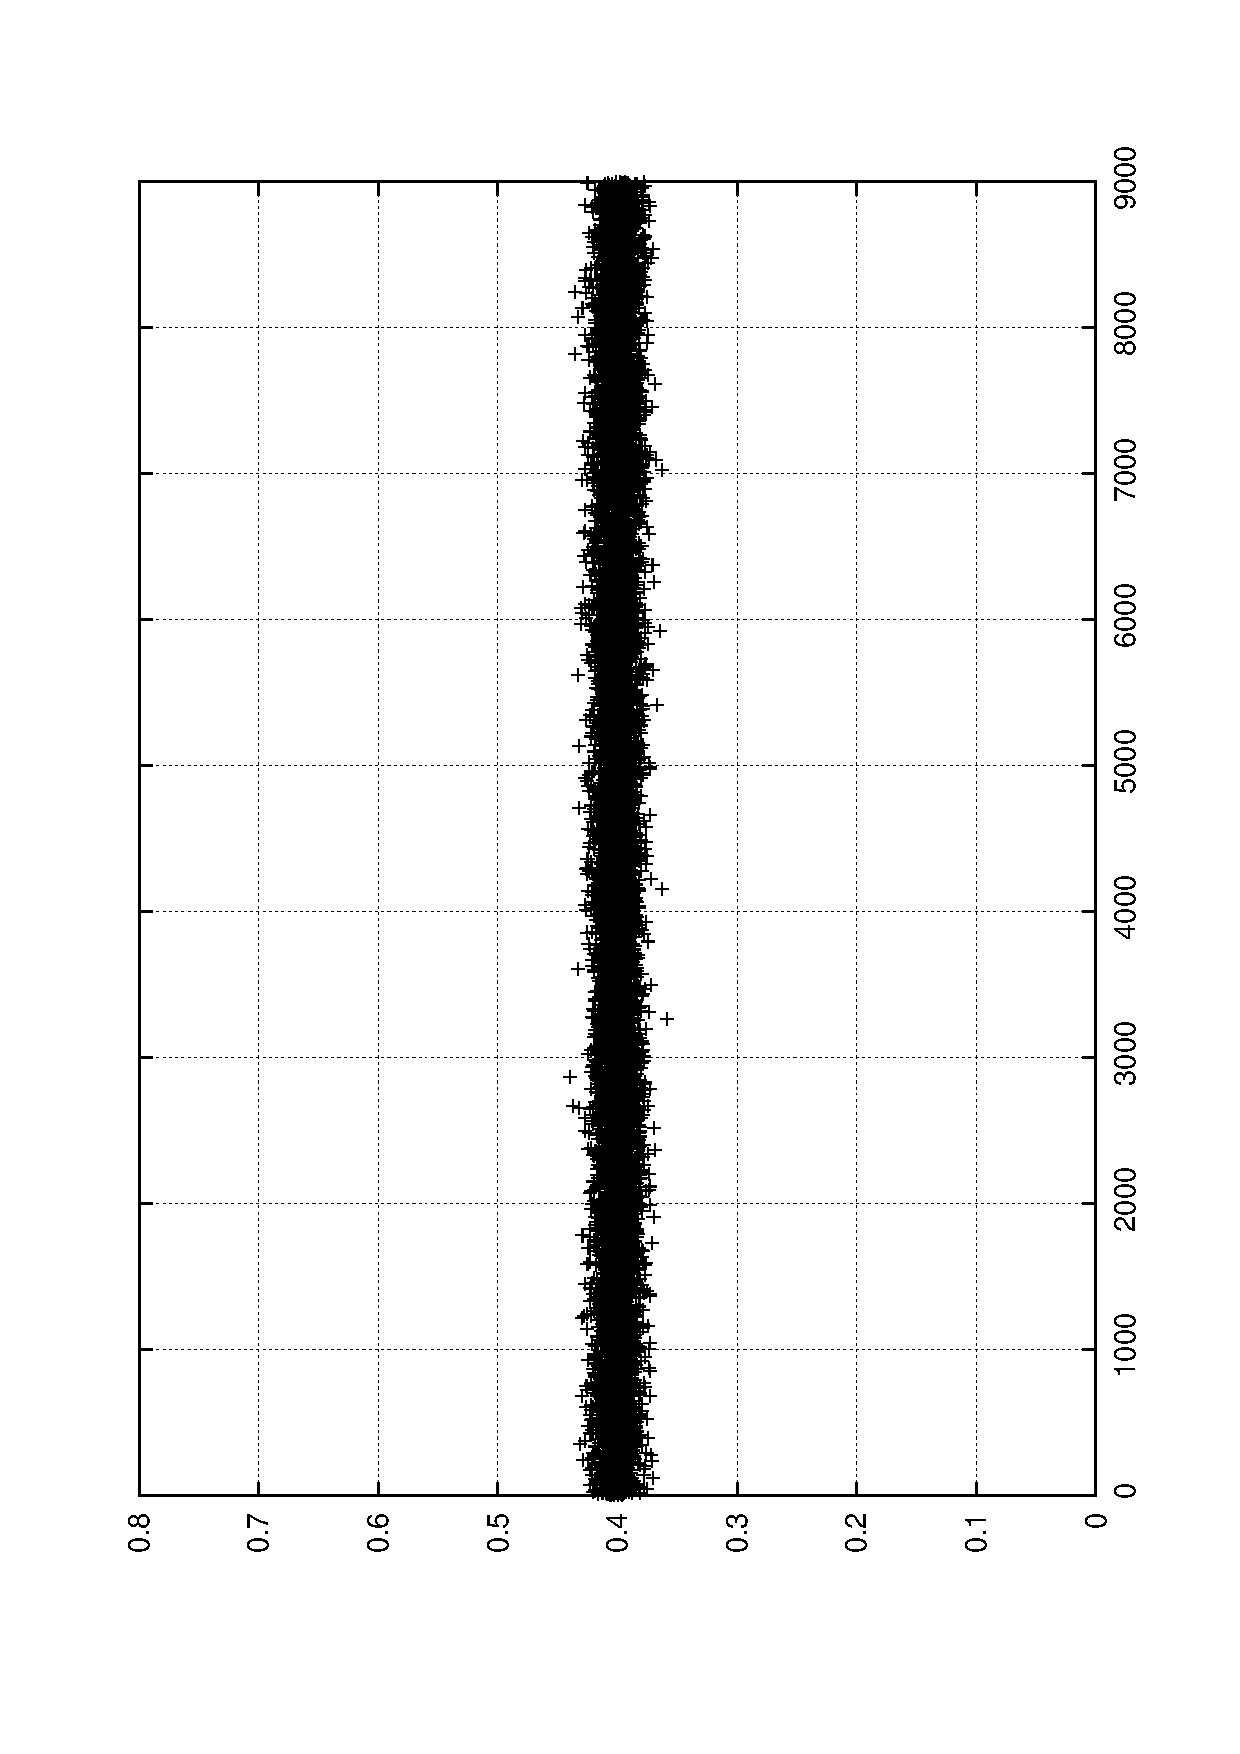
\includegraphics[scale=0.3]{trace-normal}
\end{frame}


\begin{frame}
  \frametitle{Our simulations}
  \framesubtitle{Scenarios}
  \begin{itemize}
  \item \Ldois{}: Varying the mean execution time
  \end{itemize}
  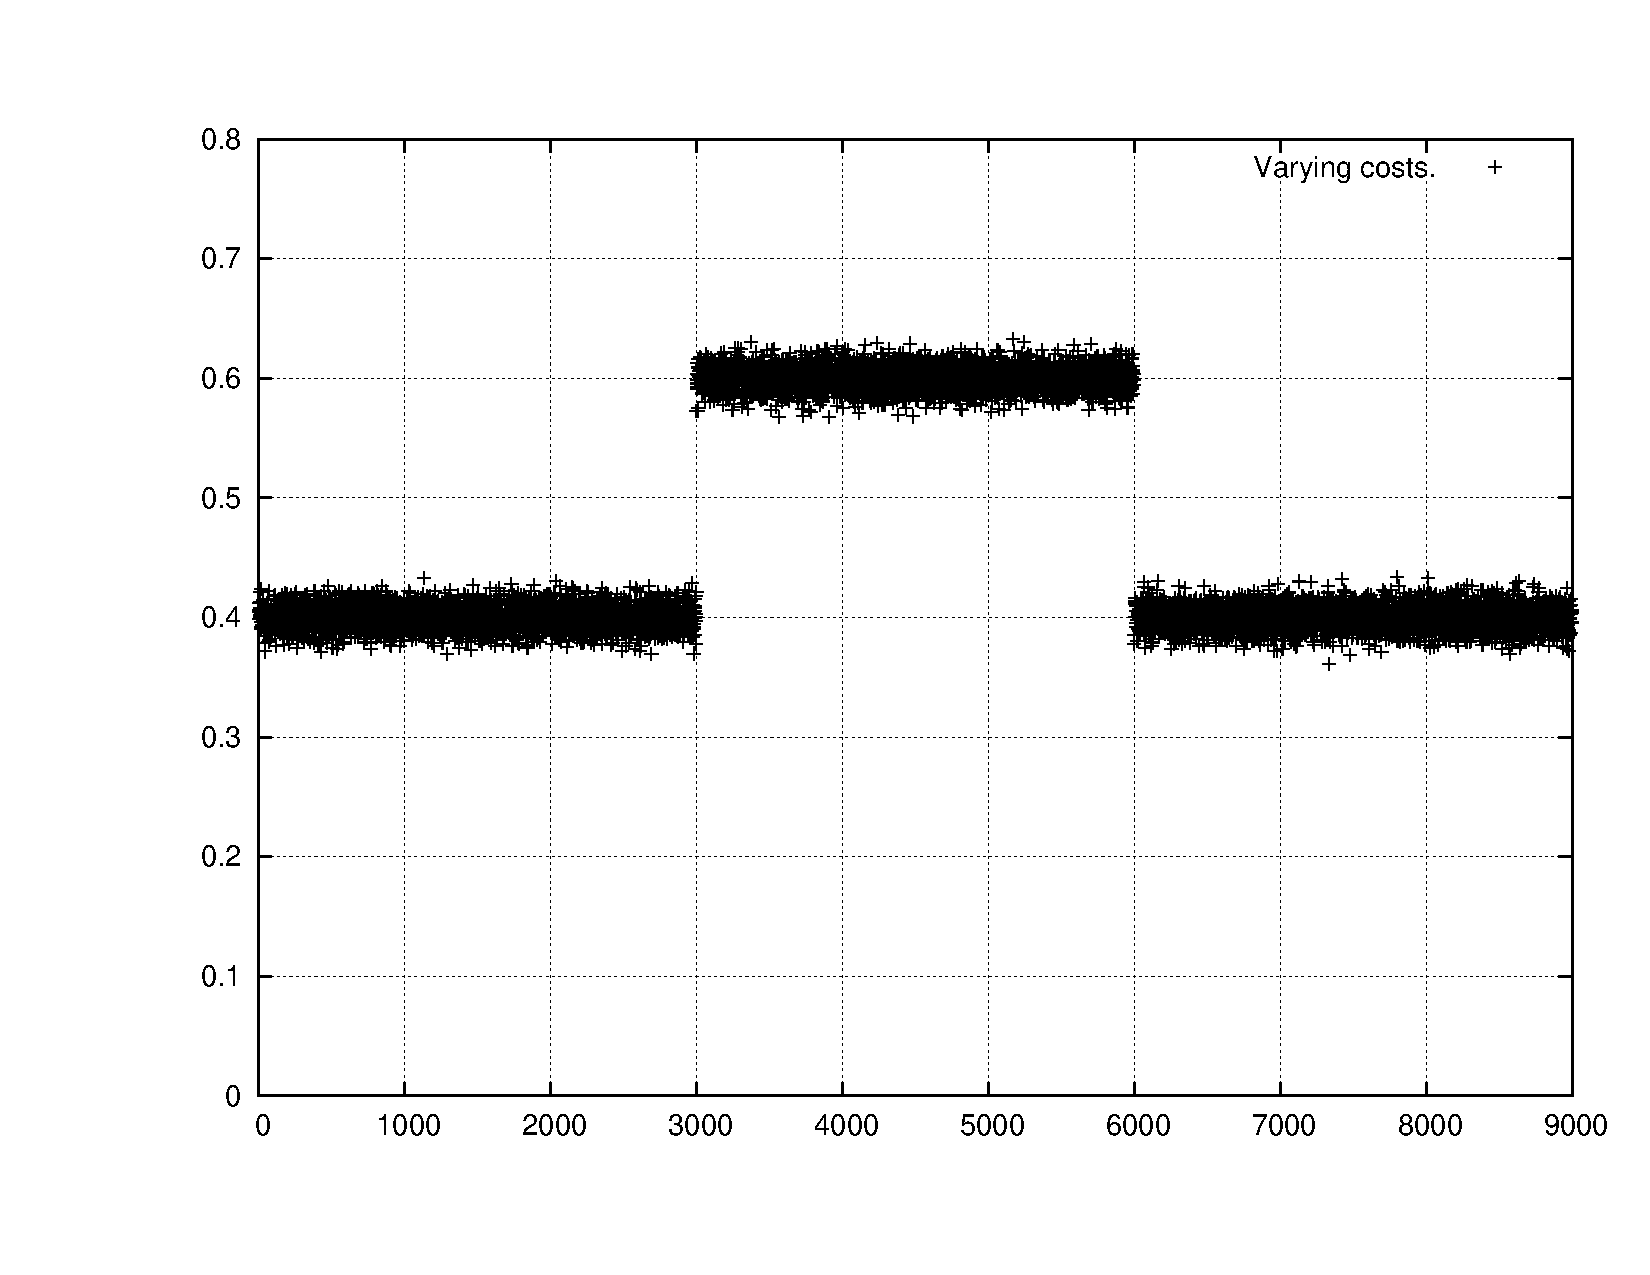
\includegraphics[scale=0.3]{trace-trifasico}
\end{frame}

\begin{frame}
  \frametitle{Our simulations}
  \framesubtitle{Scenarios}
  \begin{itemize}
  \item \Ltres{}: Varying the execution time variance
  \end{itemize}
  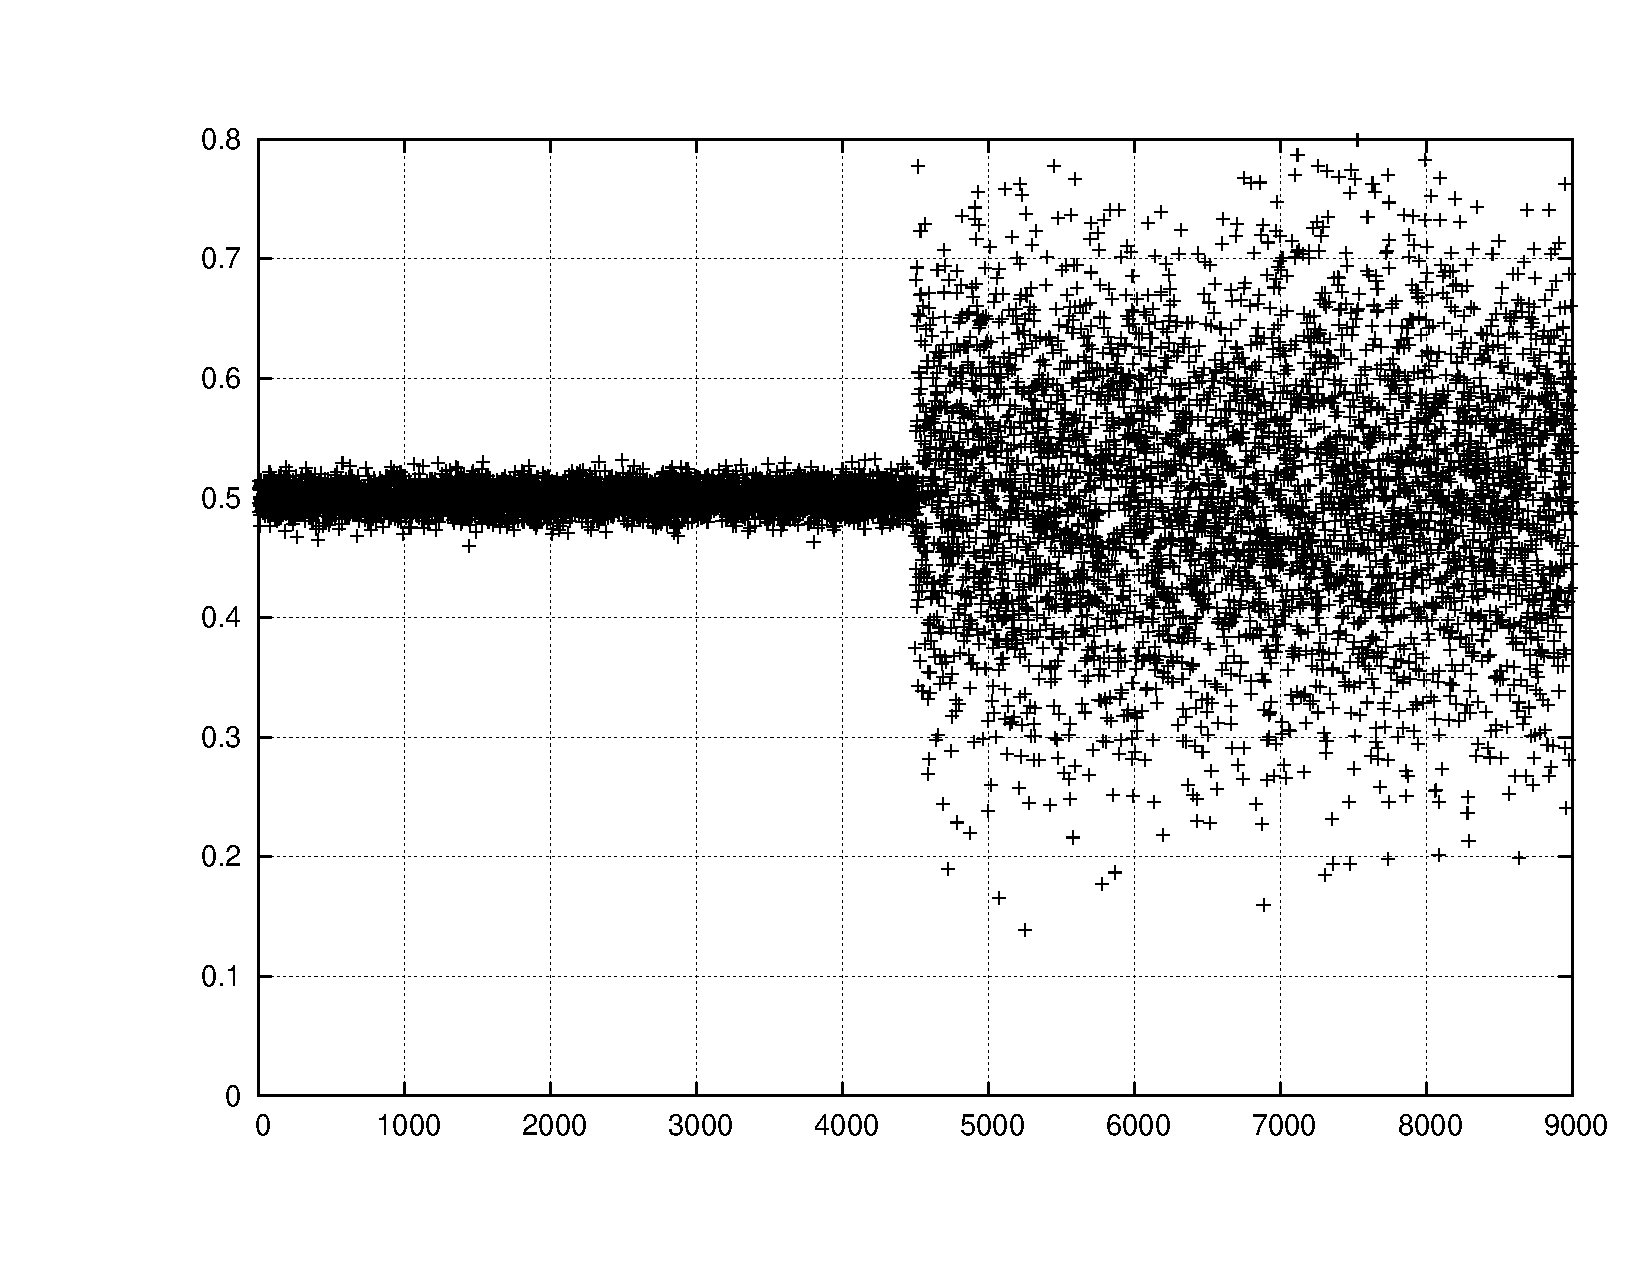
\includegraphics[scale=0.3]{trace-variance}
\end{frame}

\begin{frame}
  \frametitle{Our simulations}
  \framesubtitle{Scenarios}
  \begin{itemize}
  \item \Lquatro{}: A movie trace
  \end{itemize}
  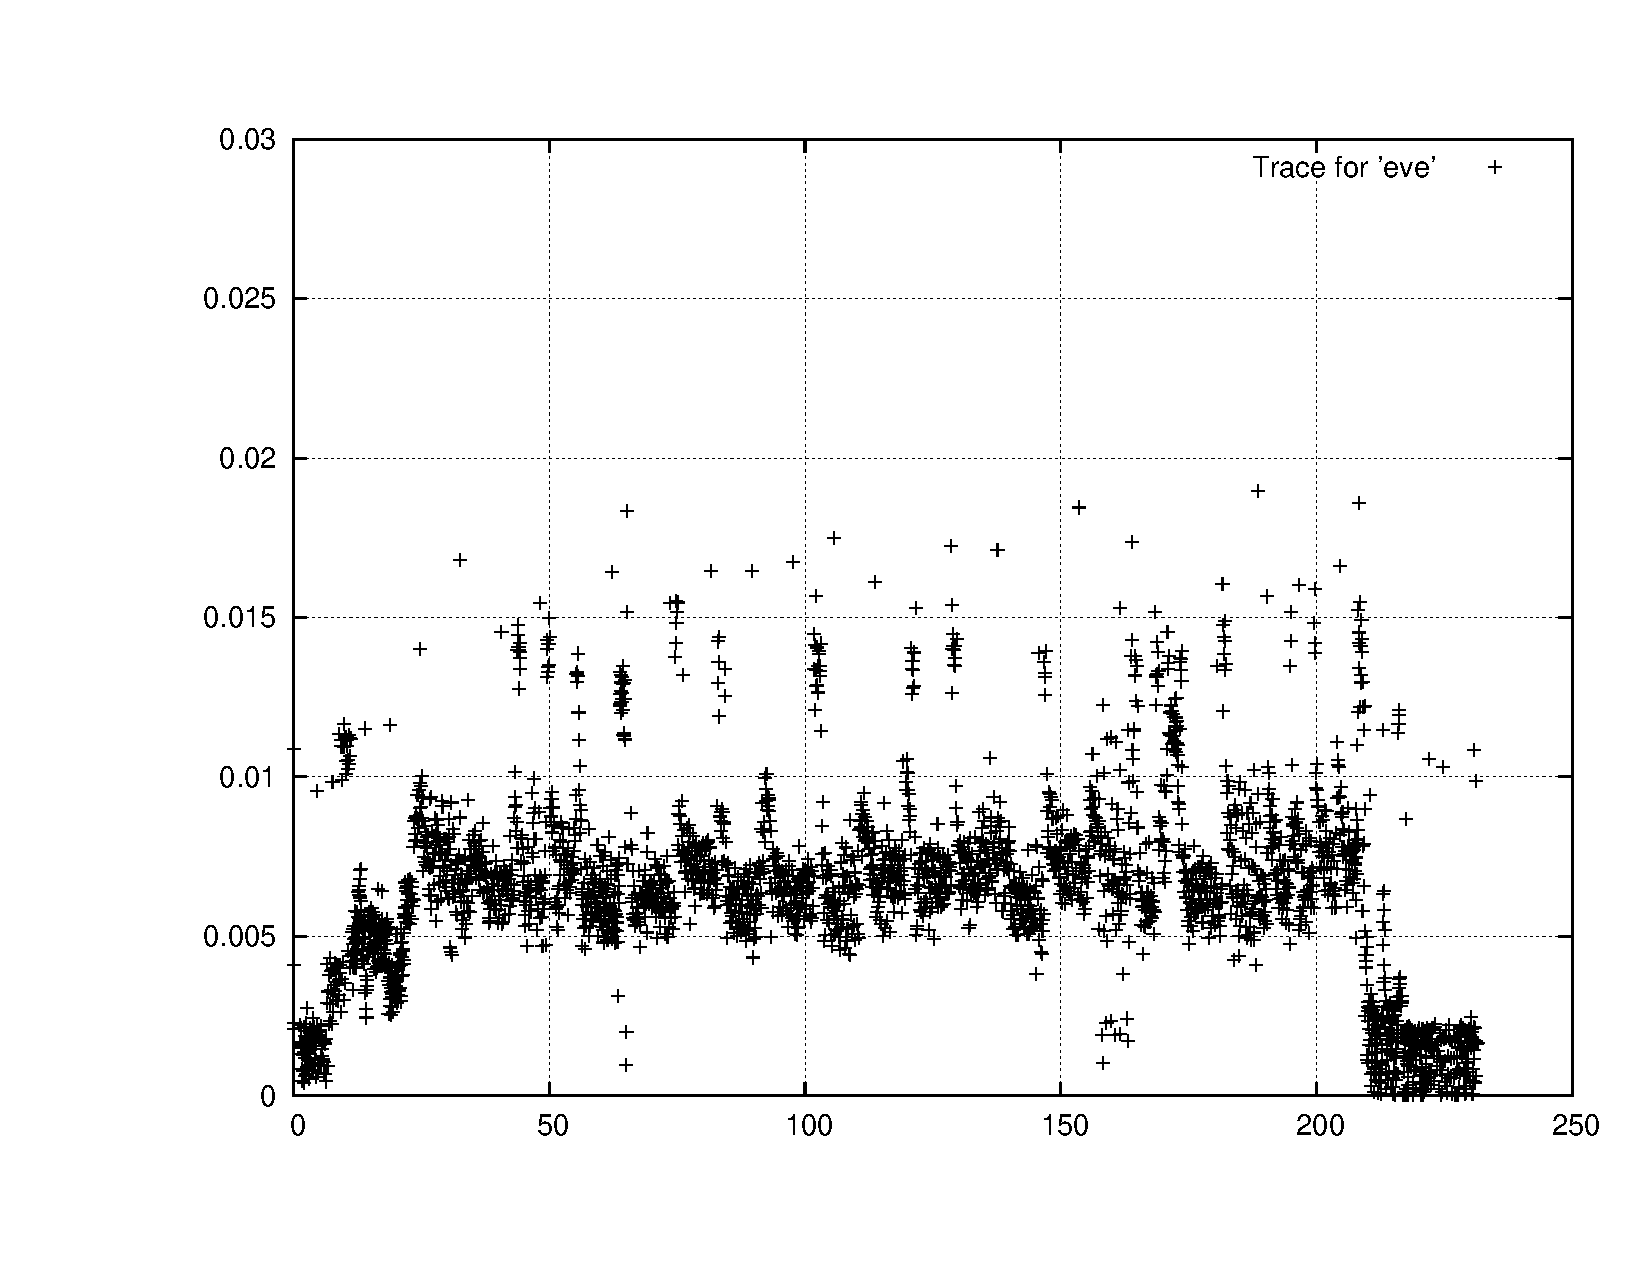
\includegraphics[scale=0.3]{trace-eve}
\end{frame}

\begin{frame}
  \frametitle{Our simulations}
  \framesubtitle{Scenarios}
  \begin{itemize}
  \item \Lcinco{}: Five movie traces at once
  \end{itemize}
  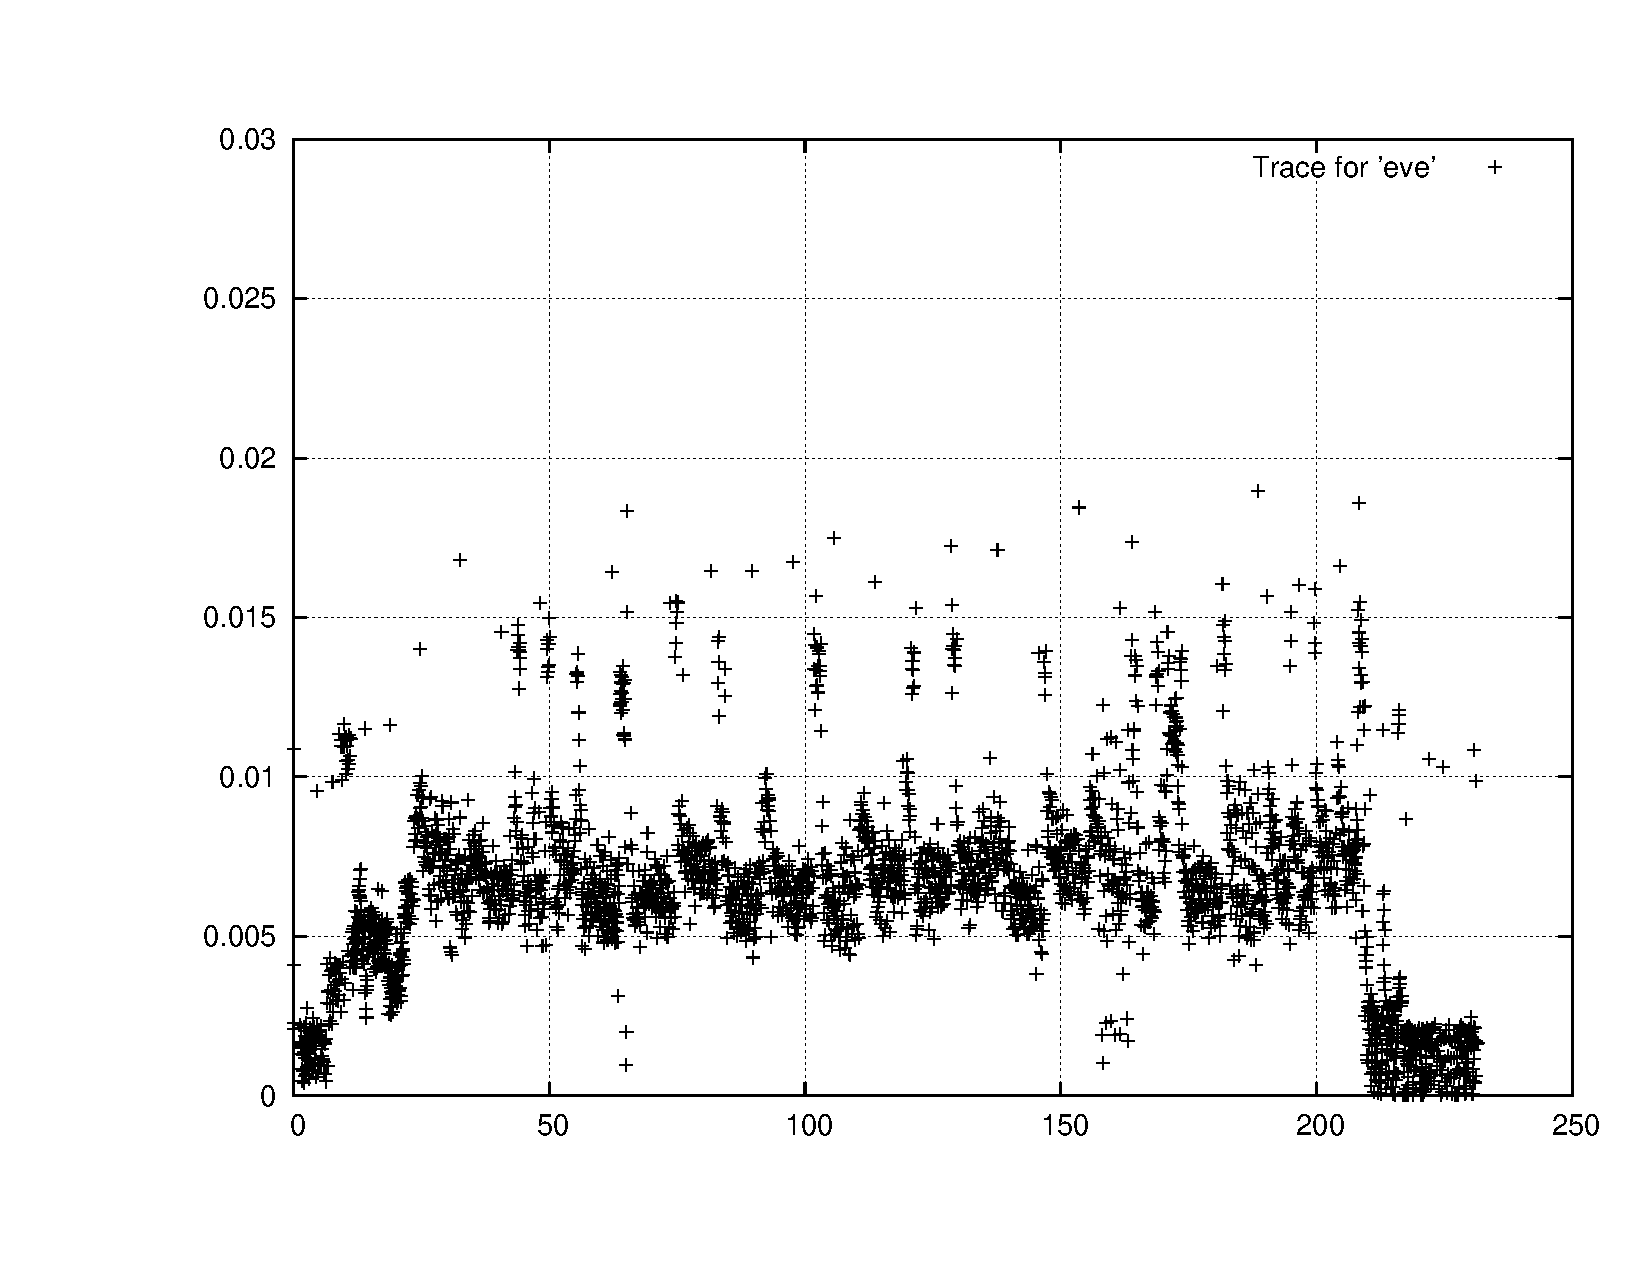
\includegraphics[scale=0.3]{trace-eve}
\end{frame}

\begin{frame}
  \frametitle{Results}
    \begin{tabular}[t]{rrrrrr} \hline
    \textsc{LS} & \textsc{RS} & \textsc{Mean RT} & \textsc{RT Jitter} & \textsc{Mean WT} & \textsc{DMR (\%)} \\ \hline
    \multirow{2}{*}{\Lum{}} & Soft & $5.1\times 10^{-1}$ & $2.3\times 10^{-1}$    & $1.1\times 10^{-1}$   & 5.4  \\
                        & Hard & $5.6\times 10^{-1}$     & $2.6\times 10^{-1}$  & $1.2\times 10^{-1}$   & 59.8 \\ \hline
    \multirow{2}{*}{\Ldois{}} & Soft & $4.8\times 10^{-1}$& $1.2\times 10^{-1}$   & $1.2\times 10^{-1}$   & 14.4 \\
                        & Hard & $4.4\times 10^{-1}$       & $1.0\times 10^{-1}$   & $1.7\times 10^{-1}$   & 37.5 \\ \hline
    \multirow{2}{*}{\Ltres{}} & Soft & $5.7\times 10^{-1}$& $1.8\times 10^{-1}$   & $8.0\times 10^{-2}$   & 5.1  \\
                        & Hard & $5.8\times 10^{-1}$       &$2.1\times 10^{-1}$    & $1.2\times 10^{-1}$   & 59.4 \\ \hline
    \multirow{2}{*}{\Lquatro{}} & Soft & $6.5\times 10^{-3}$& $4.8\times 10^{-3}$   & $3.3\times 10^{-4}$   & 0.1  \\
                        & Hard & $3.5\times 10^{-2}$       & $3.1\times 10^{-2}$   & $5.6\times 10^{-3}$   & 24.5 \\ \hline    
    \multirow{2}{*}{\Lcinco{}} & Soft & $2.5\times 10^{-3}$& $1.4\times 10^{-2}$   & $6.4\times 10^{-4}$   & 0.56  \\
                        & Hard & $3.8\times 10^{-2}$       & $2.8\times 10^{-2}$   & $1.2\times 10^{-2}$   & 23.9 \\ \hline    
  \end{tabular}
Soft reservation is universally better, on all metrics.
\end{frame}

\begin{frame}
  \frametitle{Understanding this result}
  \framesubtitle{How can the jitter be higher in hard reservation?}
    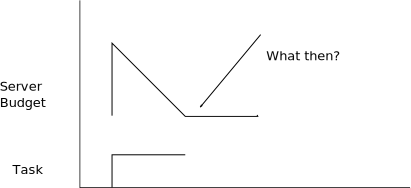
\includegraphics[scale=0.5]{hardvsoft}
    
    \vspace{1cm}
    
    If soft, the server might run soon; if hard it will wait until the
    next period to do so.
\end{frame}

\begin{frame}
  \frametitle{Understanding this result}
  \framesubtitle{How can the deadline miss ratio be higher in hard
    reservation?}
    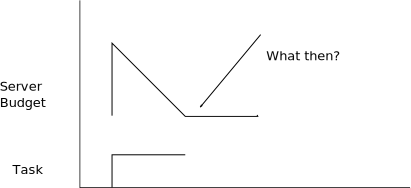
\includegraphics[scale=0.5]{hardvsoft}
    
    \vspace{1cm}
    
    When a hard server recharges its budget the task might have
    already missed its deadline.
\end{frame}

\begin{frame}
  \frametitle{Conclusions}
  \begin{itemize}
  \item Soft reservation is usually better.
  \item While hard reservation looks interesting and real-time, it
    has some hidden drawbacks that actually make it not very reliable.
  \item It is better to measure before deciding on a version to use in
    a system.
  \end{itemize}
  
\end{frame}


\end{document}